\documentclass[twoside]{book}

% Packages required by doxygen
\usepackage{fixltx2e}
\usepackage{calc}
\usepackage{doxygen}
\usepackage[export]{adjustbox} % also loads graphicx
\usepackage{graphicx}
\usepackage[utf8]{inputenc}
\usepackage{makeidx}
\usepackage{multicol}
\usepackage{multirow}
\PassOptionsToPackage{warn}{textcomp}
\usepackage{textcomp}
\usepackage[nointegrals]{wasysym}
\usepackage[table]{xcolor}

% Font selection
\usepackage[T1]{fontenc}
\usepackage[scaled=.90]{helvet}
\usepackage{courier}
\usepackage{amssymb}
\usepackage{sectsty}
\renewcommand{\familydefault}{\sfdefault}
\allsectionsfont{%
  \fontseries{bc}\selectfont%
  \color{darkgray}%
}
\renewcommand{\DoxyLabelFont}{%
  \fontseries{bc}\selectfont%
  \color{darkgray}%
}
\newcommand{\+}{\discretionary{\mbox{\scriptsize$\hookleftarrow$}}{}{}}

% Page & text layout
\usepackage{geometry}
\geometry{%
  a4paper,%
  top=2.5cm,%
  bottom=2.5cm,%
  left=2.5cm,%
  right=2.5cm%
}
\tolerance=750
\hfuzz=15pt
\hbadness=750
\setlength{\emergencystretch}{15pt}
\setlength{\parindent}{0cm}
\setlength{\parskip}{3ex plus 2ex minus 2ex}
\makeatletter
\renewcommand{\paragraph}{%
  \@startsection{paragraph}{4}{0ex}{-1.0ex}{1.0ex}{%
    \normalfont\normalsize\bfseries\SS@parafont%
  }%
}
\renewcommand{\subparagraph}{%
  \@startsection{subparagraph}{5}{0ex}{-1.0ex}{1.0ex}{%
    \normalfont\normalsize\bfseries\SS@subparafont%
  }%
}
\makeatother

% Headers & footers
\usepackage{fancyhdr}
\pagestyle{fancyplain}
\fancyhead[LE]{\fancyplain{}{\bfseries\thepage}}
\fancyhead[CE]{\fancyplain{}{}}
\fancyhead[RE]{\fancyplain{}{\bfseries\leftmark}}
\fancyhead[LO]{\fancyplain{}{\bfseries\rightmark}}
\fancyhead[CO]{\fancyplain{}{}}
\fancyhead[RO]{\fancyplain{}{\bfseries\thepage}}
\fancyfoot[LE]{\fancyplain{}{}}
\fancyfoot[CE]{\fancyplain{}{}}
\fancyfoot[RE]{\fancyplain{}{\bfseries\scriptsize Generated by Doxygen }}
\fancyfoot[LO]{\fancyplain{}{\bfseries\scriptsize Generated by Doxygen }}
\fancyfoot[CO]{\fancyplain{}{}}
\fancyfoot[RO]{\fancyplain{}{}}
\renewcommand{\footrulewidth}{0.4pt}
\renewcommand{\chaptermark}[1]{%
  \markboth{#1}{}%
}
\renewcommand{\sectionmark}[1]{%
  \markright{\thesection\ #1}%
}

% Indices & bibliography
\usepackage{natbib}
\usepackage[titles]{tocloft}
\setcounter{tocdepth}{3}
\setcounter{secnumdepth}{5}
\makeindex

% Hyperlinks (required, but should be loaded last)
\usepackage{ifpdf}
\ifpdf
  \usepackage[pdftex,pagebackref=true]{hyperref}
\else
  \usepackage[ps2pdf,pagebackref=true]{hyperref}
\fi
\hypersetup{%
  colorlinks=true,%
  linkcolor=blue,%
  citecolor=blue,%
  unicode%
}

% Custom commands
\newcommand{\clearemptydoublepage}{%
  \newpage{\pagestyle{empty}\cleardoublepage}%
}

\usepackage{caption}
\captionsetup{labelsep=space,justification=centering,font={bf},singlelinecheck=off,skip=4pt,position=top}

%===== C O N T E N T S =====

\begin{document}

% Titlepage & ToC
\hypersetup{pageanchor=false,
             bookmarksnumbered=true,
             pdfencoding=unicode
            }
\pagenumbering{alph}
\begin{titlepage}
\vspace*{7cm}
\begin{center}%
{\Large Asteroid }\\
\vspace*{1cm}
{\large Generated by Doxygen 1.8.12}\\
\end{center}
\end{titlepage}
\clearemptydoublepage
\pagenumbering{roman}
\tableofcontents
\clearemptydoublepage
\pagenumbering{arabic}
\hypersetup{pageanchor=true}

%--- Begin generated contents ---
\chapter{Template}
\label{md__r_e_a_d_m_e}
\hypertarget{md__r_e_a_d_m_e}{}
Visual Studio 2015 Templates 
\chapter{Hierarchical Index}
\section{Class Hierarchy}
This inheritance list is sorted roughly, but not completely, alphabetically\+:\begin{DoxyCompactList}
\item \contentsline{section}{C\+Base4618}{\pageref{class_c_base4618}}{}
\begin{DoxyCompactList}
\item \contentsline{section}{C\+Asteriod\+Game}{\pageref{class_c_asteriod_game}}{}
\end{DoxyCompactList}
\item \contentsline{section}{C\+Control}{\pageref{class_c_control}}{}
\item \contentsline{section}{C\+Game\+Object}{\pageref{class_c_game_object}}{}
\begin{DoxyCompactList}
\item \contentsline{section}{C\+Asteroid}{\pageref{class_c_asteroid}}{}
\item \contentsline{section}{C\+Missile}{\pageref{class_c_missile}}{}
\item \contentsline{section}{C\+Ship}{\pageref{class_c_ship}}{}
\end{DoxyCompactList}
\item \contentsline{section}{Client}{\pageref{class_client}}{}
\item \contentsline{section}{Serial}{\pageref{class_serial}}{}
\item \contentsline{section}{Server}{\pageref{class_server}}{}
\end{DoxyCompactList}

\chapter{Class Index}
\section{Class List}
Here are the classes, structs, unions and interfaces with brief descriptions\+:\begin{DoxyCompactList}
\item\contentsline{section}{\hyperlink{class_c_asteriod_game}{C\+Asteriod\+Game} \\*C++ object used draw usnig M\+S\+P432 J\+O\+T\+S\+T\+I\+CK }{\pageref{class_c_asteriod_game}}{}
\item\contentsline{section}{\hyperlink{class_c_asteroid}{C\+Asteroid} \\*C++ Asteroid object contains asteroid data }{\pageref{class_c_asteroid}}{}
\item\contentsline{section}{\hyperlink{class_c_base4618}{C\+Base4618} \\*C++ object used to hold common code used in all of the following labs for this course }{\pageref{class_c_base4618}}{}
\item\contentsline{section}{\hyperlink{class_c_control}{C\+Control} \\*C++ object used for communication with the embedded system }{\pageref{class_c_control}}{}
\item\contentsline{section}{\hyperlink{class_c_game_object}{C\+Game\+Object} \\*C++ object used to hold common code used in each object of the game }{\pageref{class_c_game_object}}{}
\item\contentsline{section}{\hyperlink{class_client}{Client} }{\pageref{class_client}}{}
\item\contentsline{section}{\hyperlink{class_c_missile}{C\+Missile} \\*C++ Missile object contains missile data }{\pageref{class_c_missile}}{}
\item\contentsline{section}{\hyperlink{class_c_ship}{C\+Ship} \\*C++ ship object contains ship data }{\pageref{class_c_ship}}{}
\item\contentsline{section}{\hyperlink{class_serial}{Serial} }{\pageref{class_serial}}{}
\item\contentsline{section}{\hyperlink{class_server}{Server} }{\pageref{class_server}}{}
\end{DoxyCompactList}

\chapter{Class Documentation}
\hypertarget{class_c_asteriod_game}{}\section{C\+Asteriod\+Game Class Reference}
\label{class_c_asteriod_game}\index{C\+Asteriod\+Game@{C\+Asteriod\+Game}}


C++ object used draw usnig M\+S\+P432 J\+O\+T\+S\+T\+I\+CK.  




{\ttfamily \#include $<$C\+Asteriod\+Game.\+h$>$}

Inheritance diagram for C\+Asteriod\+Game\+:\begin{figure}[H]
\begin{center}
\leavevmode
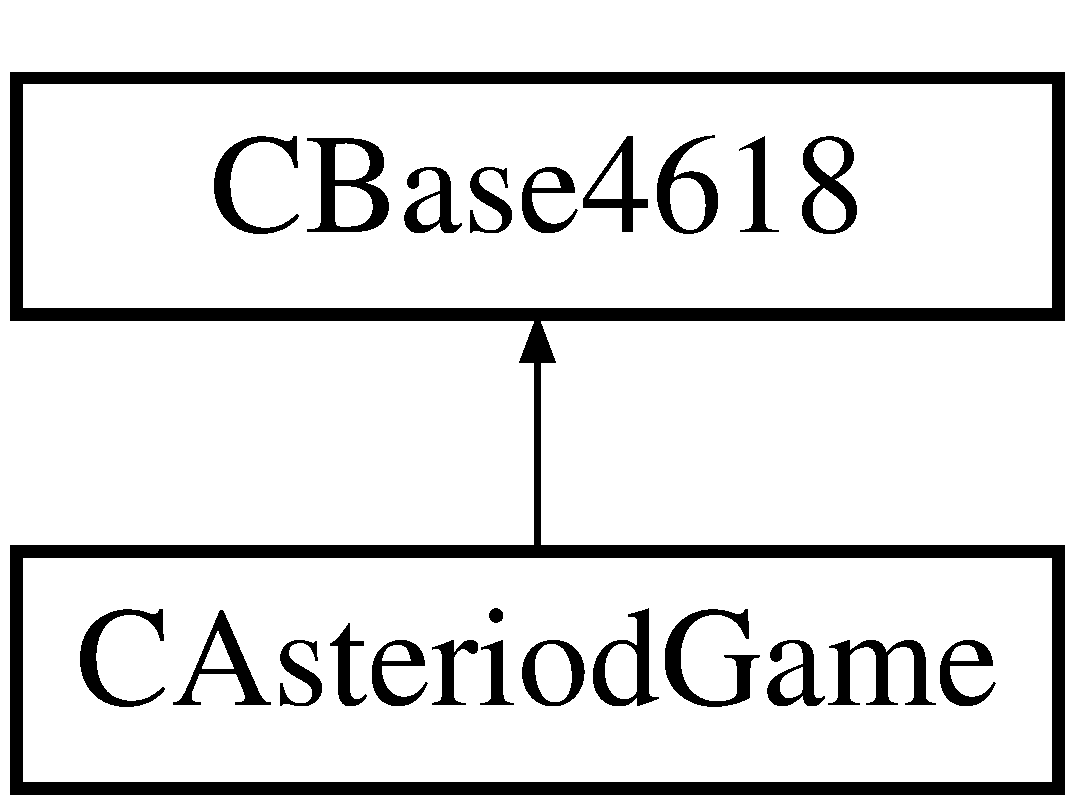
\includegraphics[height=2.000000cm]{class_c_asteriod_game}
\end{center}
\end{figure}
\subsection*{Public Member Functions}
\begin{DoxyCompactItemize}
\item 
\hyperlink{class_c_asteriod_game_afdff290987d441921d6549e8f6756b5d}{C\+Asteriod\+Game} (cv\+::\+Size d, int)
\begin{DoxyCompactList}\small\item\em Sets the desired C\+OM port. \end{DoxyCompactList}\item 
void \hyperlink{class_c_asteriod_game_abe38958a37bed1b2ed5f9b08bc0332bb}{update} () override
\begin{DoxyCompactList}\small\item\em Sets the desired C\+OM port. \end{DoxyCompactList}\item 
void \hyperlink{class_c_asteriod_game_a6c14d9f6671a0789b5738cdb5bc0af3a}{draw} () override
\begin{DoxyCompactList}\small\item\em Sets the desired C\+OM port. \end{DoxyCompactList}\item 
int \hyperlink{class_c_asteriod_game_ae0c06cee7387733f0ac1ec829a85b9a2}{missile\+\_\+button} ()
\begin{DoxyCompactList}\small\item\em Sets the desired C\+OM port. \end{DoxyCompactList}\item 
\hypertarget{class_c_asteriod_game_a6568a11921b87bf187c1e91adf3281e5}{}\label{class_c_asteriod_game_a6568a11921b87bf187c1e91adf3281e5} 
void {\bfseries reset} ()
\item 
void \hyperlink{class_c_asteriod_game_a787c6be5d95bc54c4c51b33f7da41b0a}{astroid\+\_\+creation} () override
\begin{DoxyCompactList}\small\item\em Overloaded in C\+Asteroidgame create asteroid objects. \end{DoxyCompactList}\end{DoxyCompactItemize}
\subsection*{Public Attributes}
\begin{DoxyCompactItemize}
\item 
\hypertarget{class_c_asteriod_game_a2a5b27022639d276fbfcd7c104c9ae4b}{}\label{class_c_asteriod_game_a2a5b27022639d276fbfcd7c104c9ae4b} 
\hyperlink{class_c_ship}{C\+Ship} \hyperlink{class_c_asteriod_game_a2a5b27022639d276fbfcd7c104c9ae4b}{ship}
\begin{DoxyCompactList}\small\item\em ship object \end{DoxyCompactList}\item 
\hypertarget{class_c_asteriod_game_ab3e28c412e952053ed4891d874e9da00}{}\label{class_c_asteriod_game_ab3e28c412e952053ed4891d874e9da00} 
int \hyperlink{class_c_asteriod_game_ab3e28c412e952053ed4891d874e9da00}{score} = 0
\begin{DoxyCompactList}\small\item\em keeps track of score \end{DoxyCompactList}\item 
\hypertarget{class_c_asteriod_game_ad7535a2ae585354665ac32ec6ee09d37}{}\label{class_c_asteriod_game_ad7535a2ae585354665ac32ec6ee09d37} 
int \hyperlink{class_c_asteriod_game_ad7535a2ae585354665ac32ec6ee09d37}{l}
\begin{DoxyCompactList}\small\item\em keeps track of lives \end{DoxyCompactList}\item 
\hypertarget{class_c_asteriod_game_a5514a675612ac2983fc876269ecebcfa}{}\label{class_c_asteriod_game_a5514a675612ac2983fc876269ecebcfa} 
int \hyperlink{class_c_asteriod_game_a5514a675612ac2983fc876269ecebcfa}{x\+\_\+pos}
\begin{DoxyCompactList}\small\item\em X value Jo\+Y\+S\+T\+I\+CK. \end{DoxyCompactList}\item 
\hypertarget{class_c_asteriod_game_a3ddfd0ab3410a4d07562ee198fb98694}{}\label{class_c_asteriod_game_a3ddfd0ab3410a4d07562ee198fb98694} 
int \hyperlink{class_c_asteriod_game_a3ddfd0ab3410a4d07562ee198fb98694}{y\+\_\+pos}
\begin{DoxyCompactList}\small\item\em Y value Jo\+Y\+S\+T\+I\+CK. \end{DoxyCompactList}\item 
\hypertarget{class_c_asteriod_game_aa560e4cfbc6d6d8eb4ee9d9ec4b8dbca}{}\label{class_c_asteriod_game_aa560e4cfbc6d6d8eb4ee9d9ec4b8dbca} 
int \hyperlink{class_c_asteriod_game_aa560e4cfbc6d6d8eb4ee9d9ec4b8dbca}{flag\+\_\+reset}
\begin{DoxyCompactList}\small\item\em B\+U\+T\+T\+ON F\+L\+AG value Jo\+Y\+S\+T\+I\+CK. \end{DoxyCompactList}\item 
\hypertarget{class_c_asteriod_game_a4a2aaaee14a1edd51c80da1d015a575f}{}\label{class_c_asteriod_game_a4a2aaaee14a1edd51c80da1d015a575f} 
int {\bfseries flag\+\_\+missile}
\item 
\hypertarget{class_c_asteriod_game_a5dbfb6ea22740143ef219e1b049478f9}{}\label{class_c_asteriod_game_a5dbfb6ea22740143ef219e1b049478f9} 
int \hyperlink{class_c_asteriod_game_a5dbfb6ea22740143ef219e1b049478f9}{high}
\begin{DoxyCompactList}\small\item\em canvas height \end{DoxyCompactList}\item 
\hypertarget{class_c_asteriod_game_a60f49e22c39ac4d33811b0de00aae997}{}\label{class_c_asteriod_game_a60f49e22c39ac4d33811b0de00aae997} 
int \hyperlink{class_c_asteriod_game_a60f49e22c39ac4d33811b0de00aae997}{wide}
\begin{DoxyCompactList}\small\item\em canvas width \end{DoxyCompactList}\item 
\hypertarget{class_c_asteriod_game_aa07699205c513ece3c7a0ebf30a1a3c2}{}\label{class_c_asteriod_game_aa07699205c513ece3c7a0ebf30a1a3c2} 
vector$<$ \hyperlink{class_c_asteroid}{C\+Asteroid} $>$ {\bfseries asteroid\+\_\+list}
\item 
\hypertarget{class_c_asteriod_game_a71a8f626c7905b6d3a0237c1ec5af710}{}\label{class_c_asteriod_game_a71a8f626c7905b6d3a0237c1ec5af710} 
vector$<$ \hyperlink{class_c_missile}{C\+Missile} $>$ {\bfseries missile\+\_\+list}
\item 
\hypertarget{class_c_asteriod_game_ac2e49fba581b51203cbbe09fdd9b900c}{}\label{class_c_asteriod_game_ac2e49fba581b51203cbbe09fdd9b900c} 
Point2f {\bfseries pos\+\_\+ship}
\item 
\hypertarget{class_c_asteriod_game_abca95ef453d7bf0f51d443c28379c1bd}{}\label{class_c_asteriod_game_abca95ef453d7bf0f51d443c28379c1bd} 
Point2f {\bfseries pos\+\_\+missile}
\end{DoxyCompactItemize}


\subsection{Detailed Description}
C++ object used draw usnig M\+S\+P432 J\+O\+T\+S\+T\+I\+CK. 

This class inherits methods and objects from C\+Base class. this class is overloaded to get joystick data in method update and used method draw to draw on a Open cv object

\begin{DoxyAuthor}{Author}
Balkaran Sidhu 
\end{DoxyAuthor}


\subsection{Constructor \& Destructor Documentation}
\hypertarget{class_c_asteriod_game_afdff290987d441921d6549e8f6756b5d}{}\label{class_c_asteriod_game_afdff290987d441921d6549e8f6756b5d} 
\index{C\+Asteriod\+Game@{C\+Asteriod\+Game}!C\+Asteriod\+Game@{C\+Asteriod\+Game}}
\index{C\+Asteriod\+Game@{C\+Asteriod\+Game}!C\+Asteriod\+Game@{C\+Asteriod\+Game}}
\subsubsection{\texorpdfstring{C\+Asteriod\+Game()}{CAsteriodGame()}}
{\footnotesize\ttfamily C\+Asteriod\+Game\+::\+C\+Asteriod\+Game (\begin{DoxyParamCaption}\item[{cv\+::\+Size}]{d,  }\item[{int}]{com }\end{DoxyParamCaption})}



Sets the desired C\+OM port. 


\begin{DoxyParams}{Parameters}
{\em C\+OM} & port string. \\
\hline
\end{DoxyParams}
\begin{DoxyReturn}{Returns}
nothing to return 
\end{DoxyReturn}


\subsection{Member Function Documentation}
\hypertarget{class_c_asteriod_game_a787c6be5d95bc54c4c51b33f7da41b0a}{}\label{class_c_asteriod_game_a787c6be5d95bc54c4c51b33f7da41b0a} 
\index{C\+Asteriod\+Game@{C\+Asteriod\+Game}!astroid\+\_\+creation@{astroid\+\_\+creation}}
\index{astroid\+\_\+creation@{astroid\+\_\+creation}!C\+Asteriod\+Game@{C\+Asteriod\+Game}}
\subsubsection{\texorpdfstring{astroid\+\_\+creation()}{astroid\_creation()}}
{\footnotesize\ttfamily void C\+Asteriod\+Game\+::astroid\+\_\+creation (\begin{DoxyParamCaption}{ }\end{DoxyParamCaption})\hspace{0.3cm}{\ttfamily [override]}, {\ttfamily [virtual]}}



Overloaded in C\+Asteroidgame create asteroid objects. 


\begin{DoxyParams}{Parameters}
{\em N\+O\+N\+E.} & \\
\hline
\end{DoxyParams}
\begin{DoxyReturn}{Returns}
Nothing to return 
\end{DoxyReturn}


Reimplemented from \hyperlink{class_c_base4618_a30aae55b21db35e1d70b04659a0feeb9}{C\+Base4618}.

\hypertarget{class_c_asteriod_game_a6c14d9f6671a0789b5738cdb5bc0af3a}{}\label{class_c_asteriod_game_a6c14d9f6671a0789b5738cdb5bc0af3a} 
\index{C\+Asteriod\+Game@{C\+Asteriod\+Game}!draw@{draw}}
\index{draw@{draw}!C\+Asteriod\+Game@{C\+Asteriod\+Game}}
\subsubsection{\texorpdfstring{draw()}{draw()}}
{\footnotesize\ttfamily void C\+Asteriod\+Game\+::draw (\begin{DoxyParamCaption}{ }\end{DoxyParamCaption})\hspace{0.3cm}{\ttfamily [override]}, {\ttfamily [virtual]}}



Sets the desired C\+OM port. 


\begin{DoxyParams}{Parameters}
{\em C\+OM} & port string. \\
\hline
\end{DoxyParams}
\begin{DoxyReturn}{Returns}
nothing to return 
\end{DoxyReturn}


Reimplemented from \hyperlink{class_c_base4618_a853327d563d064bb31db241861c4d291}{C\+Base4618}.

\hypertarget{class_c_asteriod_game_ae0c06cee7387733f0ac1ec829a85b9a2}{}\label{class_c_asteriod_game_ae0c06cee7387733f0ac1ec829a85b9a2} 
\index{C\+Asteriod\+Game@{C\+Asteriod\+Game}!missile\+\_\+button@{missile\+\_\+button}}
\index{missile\+\_\+button@{missile\+\_\+button}!C\+Asteriod\+Game@{C\+Asteriod\+Game}}
\subsubsection{\texorpdfstring{missile\+\_\+button()}{missile\_button()}}
{\footnotesize\ttfamily int C\+Asteriod\+Game\+::missile\+\_\+button (\begin{DoxyParamCaption}{ }\end{DoxyParamCaption})}



Sets the desired C\+OM port. 


\begin{DoxyParams}{Parameters}
{\em C\+OM} & port string. \\
\hline
\end{DoxyParams}
\begin{DoxyReturn}{Returns}
nothing to return\+Sets the desired C\+OM port.
\end{DoxyReturn}

\begin{DoxyParams}{Parameters}
{\em C\+OM} & port string. \\
\hline
\end{DoxyParams}
\begin{DoxyReturn}{Returns}
nothing to return 
\end{DoxyReturn}
\hypertarget{class_c_asteriod_game_abe38958a37bed1b2ed5f9b08bc0332bb}{}\label{class_c_asteriod_game_abe38958a37bed1b2ed5f9b08bc0332bb} 
\index{C\+Asteriod\+Game@{C\+Asteriod\+Game}!update@{update}}
\index{update@{update}!C\+Asteriod\+Game@{C\+Asteriod\+Game}}
\subsubsection{\texorpdfstring{update()}{update()}}
{\footnotesize\ttfamily void C\+Asteriod\+Game\+::update (\begin{DoxyParamCaption}{ }\end{DoxyParamCaption})\hspace{0.3cm}{\ttfamily [override]}, {\ttfamily [virtual]}}



Sets the desired C\+OM port. 


\begin{DoxyParams}{Parameters}
{\em C\+OM} & port string. \\
\hline
\end{DoxyParams}
\begin{DoxyReturn}{Returns}
nothing to return 
\end{DoxyReturn}


Reimplemented from \hyperlink{class_c_base4618_ae1ac81eaa56ded6600262c361f723cb8}{C\+Base4618}.



The documentation for this class was generated from the following files\+:\begin{DoxyCompactItemize}
\item 
C\+Asteriod\+Game.\+h\item 
C\+Asteriod\+Game.\+cpp\end{DoxyCompactItemize}

\hypertarget{class_c_asteroid}{}\section{C\+Asteroid Class Reference}
\label{class_c_asteroid}\index{C\+Asteroid@{C\+Asteroid}}


C++ Asteroid object contains asteroid data.  




{\ttfamily \#include $<$C\+Asteroid.\+h$>$}

Inheritance diagram for C\+Asteroid\+:\begin{figure}[H]
\begin{center}
\leavevmode
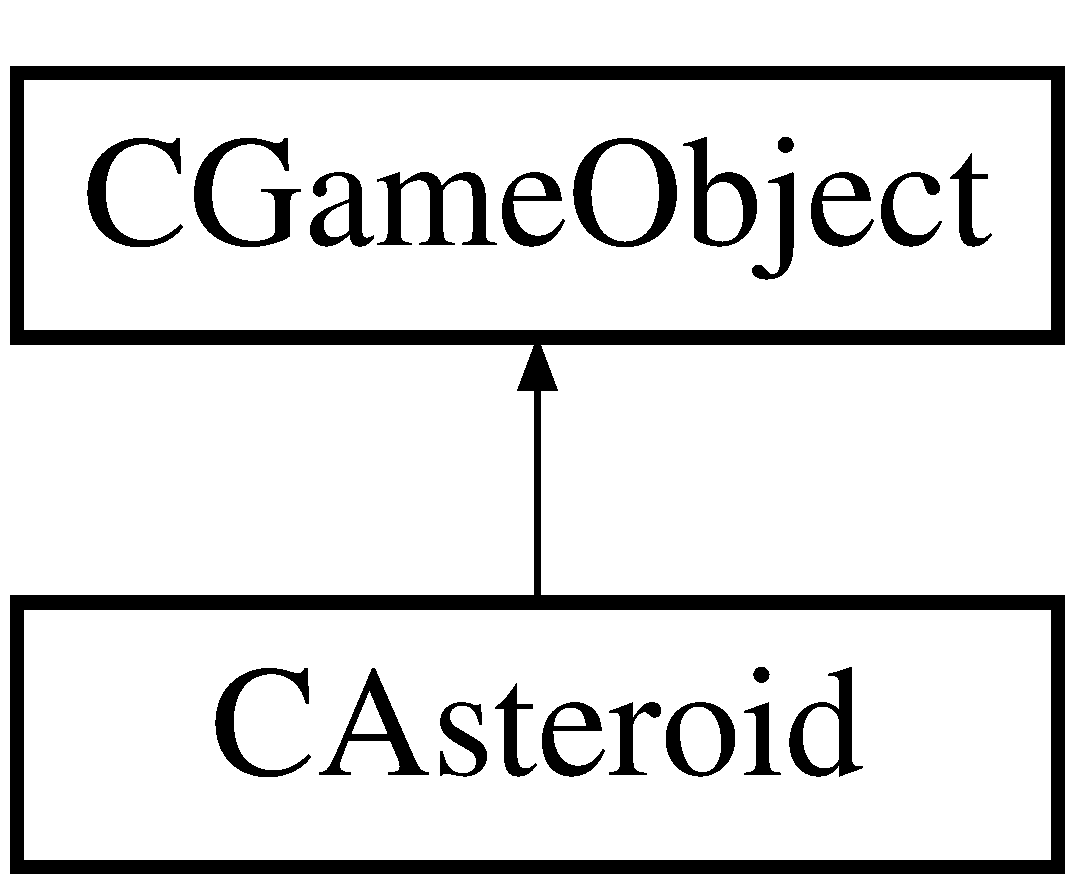
\includegraphics[height=2.000000cm]{class_c_asteroid}
\end{center}
\end{figure}
\subsection*{Public Member Functions}
\begin{DoxyCompactItemize}
\item 
\hyperlink{class_c_asteroid_a12e176ee14187759aab8c3c22b31803b}{C\+Asteroid} ()
\begin{DoxyCompactList}\small\item\em contains intial object stats. \end{DoxyCompactList}\end{DoxyCompactItemize}
\subsection*{Additional Inherited Members}


\subsection{Detailed Description}
C++ Asteroid object contains asteroid data. 

This class has a all the characteristics of a asteroid

\begin{DoxyAuthor}{Author}
Balkaran Sidhu 
\end{DoxyAuthor}


\subsection{Constructor \& Destructor Documentation}
\hypertarget{class_c_asteroid_a12e176ee14187759aab8c3c22b31803b}{}\label{class_c_asteroid_a12e176ee14187759aab8c3c22b31803b} 
\index{C\+Asteroid@{C\+Asteroid}!C\+Asteroid@{C\+Asteroid}}
\index{C\+Asteroid@{C\+Asteroid}!C\+Asteroid@{C\+Asteroid}}
\subsubsection{\texorpdfstring{C\+Asteroid()}{CAsteroid()}}
{\footnotesize\ttfamily C\+Asteroid\+::\+C\+Asteroid (\begin{DoxyParamCaption}{ }\end{DoxyParamCaption})}



contains intial object stats. 


\begin{DoxyParams}{Parameters}
{\em N\+O\+N\+E.} & \\
\hline
\end{DoxyParams}
\begin{DoxyReturn}{Returns}
nothing to return 
\end{DoxyReturn}


The documentation for this class was generated from the following files\+:\begin{DoxyCompactItemize}
\item 
C\+Asteroid.\+h\item 
C\+Asteroid.\+cpp\end{DoxyCompactItemize}

\hypertarget{class_c_base4618}{}\section{C\+Base4618 Class Reference}
\label{class_c_base4618}\index{C\+Base4618@{C\+Base4618}}


C++ object used to hold common code used in all of the following labs for this course.  




{\ttfamily \#include $<$C\+Base4618.\+h$>$}

Inheritance diagram for C\+Base4618\+:\begin{figure}[H]
\begin{center}
\leavevmode
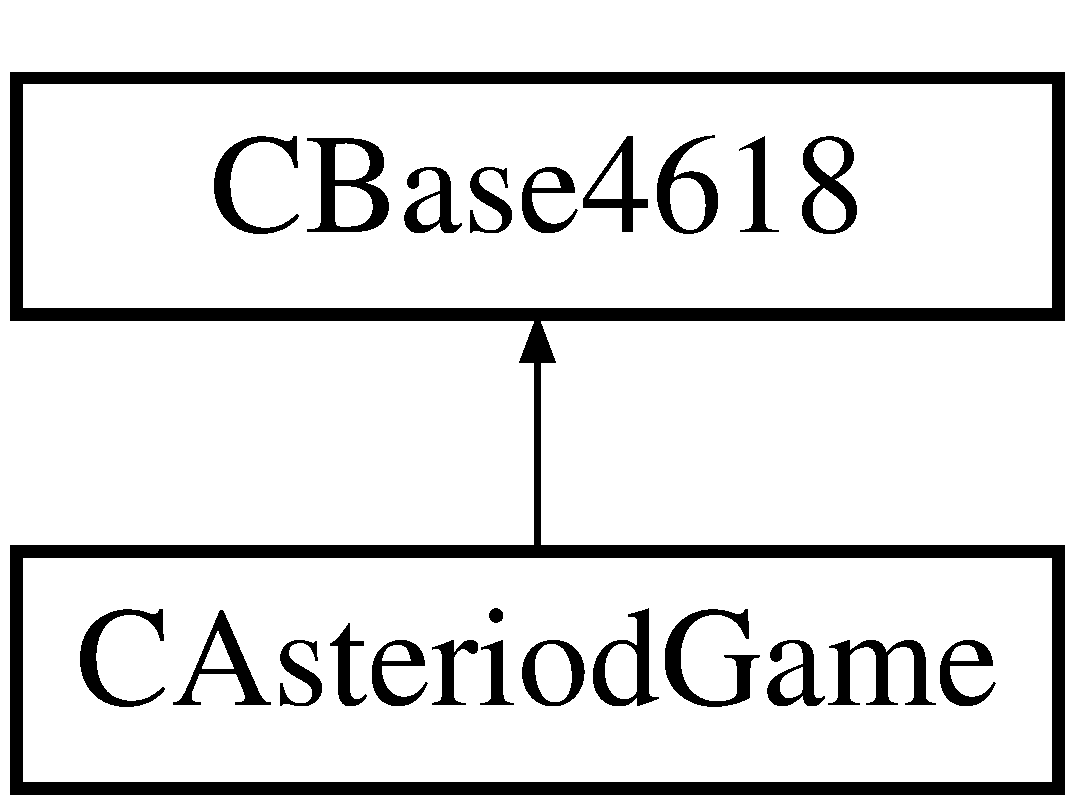
\includegraphics[height=2.000000cm]{class_c_base4618}
\end{center}
\end{figure}
\subsection*{Public Member Functions}
\begin{DoxyCompactItemize}
\item 
virtual void \hyperlink{class_c_base4618_ae1ac81eaa56ded6600262c361f723cb8}{update} ()
\begin{DoxyCompactList}\small\item\em Overloaded in C\+Asteroidgame updates the coordinates. \end{DoxyCompactList}\item 
virtual void \hyperlink{class_c_base4618_a853327d563d064bb31db241861c4d291}{draw} ()
\begin{DoxyCompactList}\small\item\em Overloaded in C\+Asteroidgame to draw. \end{DoxyCompactList}\item 
virtual void \hyperlink{class_c_base4618_a535e816d735d10d6048dd39cd893d393}{run} ()
\begin{DoxyCompactList}\small\item\em runs update and draw in an infinite loop until a button is pressed. \end{DoxyCompactList}\item 
virtual void \hyperlink{class_c_base4618_a30aae55b21db35e1d70b04659a0feeb9}{astroid\+\_\+creation} ()
\begin{DoxyCompactList}\small\item\em Overloaded in C\+Asteroidgame create asteroid objects. \end{DoxyCompactList}\end{DoxyCompactItemize}
\subsection*{Public Attributes}
\begin{DoxyCompactItemize}
\item 
\hypertarget{class_c_base4618_aa07dc8a46156de408c94acf90f46043a}{}\label{class_c_base4618_aa07dc8a46156de408c94acf90f46043a} 
\hyperlink{class_c_control}{C\+Control} \hyperlink{class_c_base4618_aa07dc8a46156de408c94acf90f46043a}{control}
\begin{DoxyCompactList}\small\item\em Control object. \end{DoxyCompactList}\item 
\hypertarget{class_c_base4618_a1b925f757247b33ca2072f777f24582d}{}\label{class_c_base4618_a1b925f757247b33ca2072f777f24582d} 
cv\+::\+Mat \hyperlink{class_c_base4618_a1b925f757247b33ca2072f777f24582d}{\+\_\+canvas}
\begin{DoxyCompactList}\small\item\em Mat object. \end{DoxyCompactList}\item 
\hypertarget{class_c_base4618_a9592c1ee1d746ebb8cbbf5389f8033ce}{}\label{class_c_base4618_a9592c1ee1d746ebb8cbbf5389f8033ce} 
int \hyperlink{class_c_base4618_a9592c1ee1d746ebb8cbbf5389f8033ce}{random} =0
\begin{DoxyCompactList}\small\item\em random number genrated \end{DoxyCompactList}\item 
\hypertarget{class_c_base4618_afdacbfdcf5e4dcbc0194f24eb1337b42}{}\label{class_c_base4618_afdacbfdcf5e4dcbc0194f24eb1337b42} 
double \hyperlink{class_c_base4618_afdacbfdcf5e4dcbc0194f24eb1337b42}{last}
\begin{DoxyCompactList}\small\item\em time when it hits run \end{DoxyCompactList}\end{DoxyCompactItemize}


\subsection{Detailed Description}
C++ object used to hold common code used in all of the following labs for this course. 

This class has a \hyperlink{class_c_control}{C\+Control} object and an Open cv object which are used in C\+Sketch class.\+There will also be three public methods which implement the two of which are overloaded in C\+Sketch.

\begin{DoxyAuthor}{Author}
Balkaran Sidhu 
\end{DoxyAuthor}


\subsection{Member Function Documentation}
\hypertarget{class_c_base4618_a30aae55b21db35e1d70b04659a0feeb9}{}\label{class_c_base4618_a30aae55b21db35e1d70b04659a0feeb9} 
\index{C\+Base4618@{C\+Base4618}!astroid\+\_\+creation@{astroid\+\_\+creation}}
\index{astroid\+\_\+creation@{astroid\+\_\+creation}!C\+Base4618@{C\+Base4618}}
\subsubsection{\texorpdfstring{astroid\+\_\+creation()}{astroid\_creation()}}
{\footnotesize\ttfamily void C\+Base4618\+::astroid\+\_\+creation (\begin{DoxyParamCaption}{ }\end{DoxyParamCaption})\hspace{0.3cm}{\ttfamily [virtual]}}



Overloaded in C\+Asteroidgame create asteroid objects. 


\begin{DoxyParams}{Parameters}
{\em N\+O\+N\+E.} & \\
\hline
\end{DoxyParams}
\begin{DoxyReturn}{Returns}
Nothing to return 
\end{DoxyReturn}


Reimplemented in \hyperlink{class_c_asteriod_game_a787c6be5d95bc54c4c51b33f7da41b0a}{C\+Asteriod\+Game}.

\hypertarget{class_c_base4618_a853327d563d064bb31db241861c4d291}{}\label{class_c_base4618_a853327d563d064bb31db241861c4d291} 
\index{C\+Base4618@{C\+Base4618}!draw@{draw}}
\index{draw@{draw}!C\+Base4618@{C\+Base4618}}
\subsubsection{\texorpdfstring{draw()}{draw()}}
{\footnotesize\ttfamily void C\+Base4618\+::draw (\begin{DoxyParamCaption}{ }\end{DoxyParamCaption})\hspace{0.3cm}{\ttfamily [virtual]}}



Overloaded in C\+Asteroidgame to draw. 


\begin{DoxyParams}{Parameters}
{\em N\+O\+N\+E.} & \\
\hline
\end{DoxyParams}
\begin{DoxyReturn}{Returns}
nothing to return 
\end{DoxyReturn}


Reimplemented in \hyperlink{class_c_asteriod_game_a6c14d9f6671a0789b5738cdb5bc0af3a}{C\+Asteriod\+Game}.

\hypertarget{class_c_base4618_a535e816d735d10d6048dd39cd893d393}{}\label{class_c_base4618_a535e816d735d10d6048dd39cd893d393} 
\index{C\+Base4618@{C\+Base4618}!run@{run}}
\index{run@{run}!C\+Base4618@{C\+Base4618}}
\subsubsection{\texorpdfstring{run()}{run()}}
{\footnotesize\ttfamily void C\+Base4618\+::run (\begin{DoxyParamCaption}{ }\end{DoxyParamCaption})\hspace{0.3cm}{\ttfamily [virtual]}}



runs update and draw in an infinite loop until a button is pressed. 


\begin{DoxyParams}{Parameters}
{\em N\+O\+N\+E.} & \\
\hline
\end{DoxyParams}
\begin{DoxyReturn}{Returns}
Nothing to return 
\end{DoxyReturn}
\hypertarget{class_c_base4618_ae1ac81eaa56ded6600262c361f723cb8}{}\label{class_c_base4618_ae1ac81eaa56ded6600262c361f723cb8} 
\index{C\+Base4618@{C\+Base4618}!update@{update}}
\index{update@{update}!C\+Base4618@{C\+Base4618}}
\subsubsection{\texorpdfstring{update()}{update()}}
{\footnotesize\ttfamily void C\+Base4618\+::update (\begin{DoxyParamCaption}{ }\end{DoxyParamCaption})\hspace{0.3cm}{\ttfamily [virtual]}}



Overloaded in C\+Asteroidgame updates the coordinates. 


\begin{DoxyParams}{Parameters}
{\em None.} & \\
\hline
\end{DoxyParams}
\begin{DoxyReturn}{Returns}
nothing to return 
\end{DoxyReturn}


Reimplemented in \hyperlink{class_c_asteriod_game_abe38958a37bed1b2ed5f9b08bc0332bb}{C\+Asteriod\+Game}.



The documentation for this class was generated from the following files\+:\begin{DoxyCompactItemize}
\item 
C\+Base4618.\+h\item 
C\+Base4618.\+cpp\end{DoxyCompactItemize}

\hypertarget{class_c_control}{}\section{C\+Control Class Reference}
\label{class_c_control}\index{C\+Control@{C\+Control}}


C++ object used for communication with the embedded system.  




{\ttfamily \#include $<$C\+Control.\+h$>$}

\subsection*{Public Member Functions}
\begin{DoxyCompactItemize}
\item 
void \hyperlink{class_c_control_a96db7512a2239f017fc27354eb840abf}{init\+\_\+com} (int com)
\begin{DoxyCompactList}\small\item\em Sets the desired C\+OM port. \end{DoxyCompactList}\item 
bool \hyperlink{class_c_control_a08d481253181db60a8aec73583a1713f}{get\+\_\+data} (string mode, string type, string channel, int \&result)
\begin{DoxyCompactList}\small\item\em Gets data on a digital or analog channel. \end{DoxyCompactList}\item 
bool \hyperlink{class_c_control_a96b82a830c7dca2ee4fd66f5c04d0c9a}{set\+\_\+data} (string type, string channel, string val)
\begin{DoxyCompactList}\small\item\em S\+E\+Ts data on a digital channel. \end{DoxyCompactList}\item 
int \hyperlink{class_c_control_acf0620145af8af25d74656b0e66e8658}{get\+\_\+analog} (int value)
\begin{DoxyCompactList}\small\item\em Returns a percent scale value of the joystick position. \end{DoxyCompactList}\item 
int \hyperlink{class_c_control_afae6ad2b10c7afb9c627e7824f30ff42}{get\+\_\+button} ()
\begin{DoxyCompactList}\small\item\em Debounces the puch button. \end{DoxyCompactList}\item 
void \hyperlink{class_c_control_a1a643d9630738943580882ea97e4caec}{servo} ()
\begin{DoxyCompactList}\small\item\em Displayes servo position. \end{DoxyCompactList}\end{DoxyCompactItemize}
\subsection*{Public Attributes}
\begin{DoxyCompactItemize}
\item 
\hypertarget{class_c_control_ace18c1c2a9b70a663bad4ede2556a788}{}\label{class_c_control_ace18c1c2a9b70a663bad4ede2556a788} 
int \hyperlink{class_c_control_ace18c1c2a9b70a663bad4ede2556a788}{x}
\begin{DoxyCompactList}\small\item\em X value Jo\+Y\+S\+T\+I\+CK. \end{DoxyCompactList}\item 
\hypertarget{class_c_control_a143a30a147cb0e1487ff52a7ca1a937e}{}\label{class_c_control_a143a30a147cb0e1487ff52a7ca1a937e} 
int \hyperlink{class_c_control_a143a30a147cb0e1487ff52a7ca1a937e}{y}
\begin{DoxyCompactList}\small\item\em Y vakue J\+O\+Y\+S\+T\+I\+CK. \end{DoxyCompactList}\end{DoxyCompactItemize}


\subsection{Detailed Description}
C++ object used for communication with the embedded system. 

This class has a serial port object and an init\+\_\+com method which initializes the serial port to the com port passed as a parameter to the method.\+There will also be two public methods which implement the serial communication protocol

\begin{DoxyAuthor}{Author}
Balkaran Sidhu 
\end{DoxyAuthor}


\subsection{Member Function Documentation}
\hypertarget{class_c_control_acf0620145af8af25d74656b0e66e8658}{}\label{class_c_control_acf0620145af8af25d74656b0e66e8658} 
\index{C\+Control@{C\+Control}!get\+\_\+analog@{get\+\_\+analog}}
\index{get\+\_\+analog@{get\+\_\+analog}!C\+Control@{C\+Control}}
\subsubsection{\texorpdfstring{get\+\_\+analog()}{get\_analog()}}
{\footnotesize\ttfamily int C\+Control\+::get\+\_\+analog (\begin{DoxyParamCaption}\item[{int}]{value }\end{DoxyParamCaption})}



Returns a percent scale value of the joystick position. 


\begin{DoxyParams}{Parameters}
{\em integer} & value\+:raw value of joystick.\\
\hline
\end{DoxyParams}
\begin{DoxyReturn}{Returns}
returns percent scale value. 
\end{DoxyReturn}
\hypertarget{class_c_control_afae6ad2b10c7afb9c627e7824f30ff42}{}\label{class_c_control_afae6ad2b10c7afb9c627e7824f30ff42} 
\index{C\+Control@{C\+Control}!get\+\_\+button@{get\+\_\+button}}
\index{get\+\_\+button@{get\+\_\+button}!C\+Control@{C\+Control}}
\subsubsection{\texorpdfstring{get\+\_\+button()}{get\_button()}}
{\footnotesize\ttfamily int C\+Control\+::get\+\_\+button (\begin{DoxyParamCaption}{ }\end{DoxyParamCaption})}



Debounces the puch button. 


\begin{DoxyParams}{Parameters}
{\em none.} & \\
\hline
\end{DoxyParams}
\begin{DoxyReturn}{Returns}
nothing to return. 
\end{DoxyReturn}
\hypertarget{class_c_control_a08d481253181db60a8aec73583a1713f}{}\label{class_c_control_a08d481253181db60a8aec73583a1713f} 
\index{C\+Control@{C\+Control}!get\+\_\+data@{get\+\_\+data}}
\index{get\+\_\+data@{get\+\_\+data}!C\+Control@{C\+Control}}
\subsubsection{\texorpdfstring{get\+\_\+data()}{get\_data()}}
{\footnotesize\ttfamily bool C\+Control\+::get\+\_\+data (\begin{DoxyParamCaption}\item[{string}]{mode,  }\item[{string}]{type,  }\item[{string}]{channel,  }\item[{int \&}]{result }\end{DoxyParamCaption})}



Gets data on a digital or analog channel. 


\begin{DoxyParams}{Parameters}
{\em strings} & of Mode used to select G\+ET or S\+ET. \\
\hline
{\em strings} & of type used to select Digital,Analog or Servo. \\
\hline
{\em strings} & of channel used select the the channel to read from. \\
\hline
{\em strings} & of result passed by referance. \\
\hline
\end{DoxyParams}
\begin{DoxyReturn}{Returns}
returns T\+R\+UE or F\+A\+L\+SE 
\end{DoxyReturn}
\hypertarget{class_c_control_a96db7512a2239f017fc27354eb840abf}{}\label{class_c_control_a96db7512a2239f017fc27354eb840abf} 
\index{C\+Control@{C\+Control}!init\+\_\+com@{init\+\_\+com}}
\index{init\+\_\+com@{init\+\_\+com}!C\+Control@{C\+Control}}
\subsubsection{\texorpdfstring{init\+\_\+com()}{init\_com()}}
{\footnotesize\ttfamily void C\+Control\+::init\+\_\+com (\begin{DoxyParamCaption}\item[{int}]{com }\end{DoxyParamCaption})}



Sets the desired C\+OM port. 


\begin{DoxyParams}{Parameters}
{\em C\+OM} & port string. \\
\hline
\end{DoxyParams}
\begin{DoxyReturn}{Returns}
nothing to return 
\end{DoxyReturn}
\hypertarget{class_c_control_a1a643d9630738943580882ea97e4caec}{}\label{class_c_control_a1a643d9630738943580882ea97e4caec} 
\index{C\+Control@{C\+Control}!servo@{servo}}
\index{servo@{servo}!C\+Control@{C\+Control}}
\subsubsection{\texorpdfstring{servo()}{servo()}}
{\footnotesize\ttfamily void C\+Control\+::servo (\begin{DoxyParamCaption}{ }\end{DoxyParamCaption})}



Displayes servo position. 


\begin{DoxyParams}{Parameters}
{\em none.} & \\
\hline
\end{DoxyParams}
\begin{DoxyReturn}{Returns}
nothing to return. 
\end{DoxyReturn}
\hypertarget{class_c_control_a96b82a830c7dca2ee4fd66f5c04d0c9a}{}\label{class_c_control_a96b82a830c7dca2ee4fd66f5c04d0c9a} 
\index{C\+Control@{C\+Control}!set\+\_\+data@{set\+\_\+data}}
\index{set\+\_\+data@{set\+\_\+data}!C\+Control@{C\+Control}}
\subsubsection{\texorpdfstring{set\+\_\+data()}{set\_data()}}
{\footnotesize\ttfamily bool C\+Control\+::set\+\_\+data (\begin{DoxyParamCaption}\item[{string}]{type,  }\item[{string}]{channel,  }\item[{string}]{val }\end{DoxyParamCaption})}



S\+E\+Ts data on a digital channel. 


\begin{DoxyParams}{Parameters}
{\em strings} & of type used to select Digital,Analog or Servo. \\
\hline
{\em strings} & of channel used select the the channel to write to. \\
\hline
{\em strings} & of valued on a channel used select the the channel to write to. \\
\hline
\end{DoxyParams}
\begin{DoxyReturn}{Returns}
returns T\+R\+UE or F\+A\+L\+SE 
\end{DoxyReturn}


The documentation for this class was generated from the following files\+:\begin{DoxyCompactItemize}
\item 
C\+Control.\+h\item 
C\+Control.\+cpp\end{DoxyCompactItemize}

\hypertarget{class_c_game_object}{}\section{C\+Game\+Object Class Reference}
\label{class_c_game_object}\index{C\+Game\+Object@{C\+Game\+Object}}


C++ object used to hold common code used in each object of the game.  




{\ttfamily \#include $<$C\+Game\+Object.\+h$>$}

Inheritance diagram for C\+Game\+Object\+:\begin{figure}[H]
\begin{center}
\leavevmode
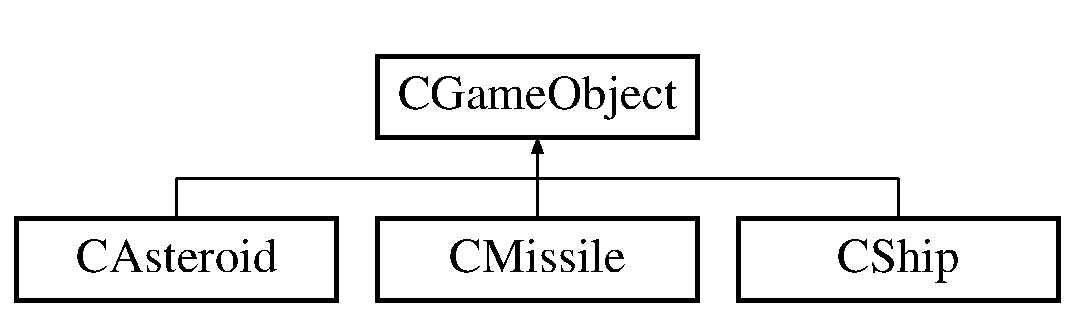
\includegraphics[height=2.000000cm]{class_c_game_object}
\end{center}
\end{figure}
\subsection*{Public Member Functions}
\begin{DoxyCompactItemize}
\item 
void \hyperlink{class_c_game_object_a5fecb17a62f57564f27a5e1120721e12}{move} ()
\begin{DoxyCompactList}\small\item\em Moves the objects. \end{DoxyCompactList}\item 
bool \hyperlink{class_c_game_object_a095ec5e8e92a7442f444a1d3b7e200da}{collide} (\hyperlink{class_c_game_object}{C\+Game\+Object} \&obj)
\begin{DoxyCompactList}\small\item\em detects collision between objects. \end{DoxyCompactList}\item 
bool \hyperlink{class_c_game_object_af1e3da2a3e10a0c11c090056eb0d027e}{collide\+\_\+wall} (Size board)
\begin{DoxyCompactList}\small\item\em detects collision with wall. \end{DoxyCompactList}\item 
void \hyperlink{class_c_game_object_ab66892d3d3db14c4b7e427f341c949dd}{hit} ()
\begin{DoxyCompactList}\small\item\em reduces lives by one after hit. \end{DoxyCompactList}\item 
int \hyperlink{class_c_game_object_a9c794264bb1c37231f137b0df3a8ccbc}{get\+\_\+lives} ()
\begin{DoxyCompactList}\small\item\em Gives the lives of the object. \end{DoxyCompactList}\item 
void \hyperlink{class_c_game_object_a1fbab5676bc0491dd10266bce54ad577}{set\+\_\+lives} (int lives)
\begin{DoxyCompactList}\small\item\em sets the lives of the object. \end{DoxyCompactList}\item 
void \hyperlink{class_c_game_object_a30b40c39c694e618e77b7c74fbd490cd}{set\+\_\+pos} (Point2f pos)
\begin{DoxyCompactList}\small\item\em Sets the position of the object. \end{DoxyCompactList}\item 
Point2f \hyperlink{class_c_game_object_a065bd87e038fcbf7c84694a426b16773}{get\+\_\+pos} ()
\begin{DoxyCompactList}\small\item\em gets the position of the object. \end{DoxyCompactList}\item 
void \hyperlink{class_c_game_object_a4cb82332eb6e3e8878eb911f6d431ebe}{draw} (Mat \&im)
\begin{DoxyCompactList}\small\item\em Draws circle . \end{DoxyCompactList}\end{DoxyCompactItemize}
\subsection*{Protected Attributes}
\begin{DoxyCompactItemize}
\item 
\hypertarget{class_c_game_object_a3ea1468f22aa6b2ef0c8cbac6e80d67a}{}\label{class_c_game_object_a3ea1468f22aa6b2ef0c8cbac6e80d67a} 
Point2f \hyperlink{class_c_game_object_a3ea1468f22aa6b2ef0c8cbac6e80d67a}{\+\_\+position}
\begin{DoxyCompactList}\small\item\em position of Object \end{DoxyCompactList}\item 
\hypertarget{class_c_game_object_a940912010105dd6890bea0a41d3a1075}{}\label{class_c_game_object_a940912010105dd6890bea0a41d3a1075} 
Point2f \hyperlink{class_c_game_object_a940912010105dd6890bea0a41d3a1075}{\+\_\+velocity}
\begin{DoxyCompactList}\small\item\em velocity of Object \end{DoxyCompactList}\item 
\hypertarget{class_c_game_object_a75ee23a373ce4a33863de12f42c8ab55}{}\label{class_c_game_object_a75ee23a373ce4a33863de12f42c8ab55} 
int \hyperlink{class_c_game_object_a75ee23a373ce4a33863de12f42c8ab55}{\+\_\+radius}
\begin{DoxyCompactList}\small\item\em radius of Object \end{DoxyCompactList}\item 
\hypertarget{class_c_game_object_acb7176fe06c83819114f7e8a8490c755}{}\label{class_c_game_object_acb7176fe06c83819114f7e8a8490c755} 
int \hyperlink{class_c_game_object_acb7176fe06c83819114f7e8a8490c755}{\+\_\+lives}
\begin{DoxyCompactList}\small\item\em lives of Object \end{DoxyCompactList}\item 
\hypertarget{class_c_game_object_aa7ebae2de18fb2b8f9cb0e6415b21552}{}\label{class_c_game_object_aa7ebae2de18fb2b8f9cb0e6415b21552} 
double \hyperlink{class_c_game_object_aa7ebae2de18fb2b8f9cb0e6415b21552}{last}
\begin{DoxyCompactList}\small\item\em previous time before move \end{DoxyCompactList}\item 
\hypertarget{class_c_game_object_aeb7a7881235150105842e90e1156b0df}{}\label{class_c_game_object_aeb7a7881235150105842e90e1156b0df} 
int \hyperlink{class_c_game_object_aeb7a7881235150105842e90e1156b0df}{B\+L\+UE}
\begin{DoxyCompactList}\small\item\em blue color of object \end{DoxyCompactList}\item 
\hypertarget{class_c_game_object_a50fdf0e7aa14e28561fe1a61d3287d38}{}\label{class_c_game_object_a50fdf0e7aa14e28561fe1a61d3287d38} 
int \hyperlink{class_c_game_object_a50fdf0e7aa14e28561fe1a61d3287d38}{G\+R\+E\+EN}
\begin{DoxyCompactList}\small\item\em green color of Object \end{DoxyCompactList}\item 
\hypertarget{class_c_game_object_aabc5155062cb7bfdee1ebce8f2d6ff76}{}\label{class_c_game_object_aabc5155062cb7bfdee1ebce8f2d6ff76} 
int \hyperlink{class_c_game_object_aabc5155062cb7bfdee1ebce8f2d6ff76}{R\+ED}
\begin{DoxyCompactList}\small\item\em red color of Object \end{DoxyCompactList}\end{DoxyCompactItemize}


\subsection{Detailed Description}
C++ object used to hold common code used in each object of the game. 

This class has a all the characteristics on all objects for example lives, size and position velocity.

\begin{DoxyAuthor}{Author}
Balkaran Sidhu 
\end{DoxyAuthor}


\subsection{Member Function Documentation}
\hypertarget{class_c_game_object_a095ec5e8e92a7442f444a1d3b7e200da}{}\label{class_c_game_object_a095ec5e8e92a7442f444a1d3b7e200da} 
\index{C\+Game\+Object@{C\+Game\+Object}!collide@{collide}}
\index{collide@{collide}!C\+Game\+Object@{C\+Game\+Object}}
\subsubsection{\texorpdfstring{collide()}{collide()}}
{\footnotesize\ttfamily bool C\+Game\+Object\+::collide (\begin{DoxyParamCaption}\item[{\hyperlink{class_c_game_object}{C\+Game\+Object} \&}]{obj }\end{DoxyParamCaption})}



detects collision between objects. 


\begin{DoxyParams}{Parameters}
{\em a} & game object for example asteroid. \\
\hline
\end{DoxyParams}
\begin{DoxyReturn}{Returns}
True or False 
\end{DoxyReturn}
\hypertarget{class_c_game_object_af1e3da2a3e10a0c11c090056eb0d027e}{}\label{class_c_game_object_af1e3da2a3e10a0c11c090056eb0d027e} 
\index{C\+Game\+Object@{C\+Game\+Object}!collide\+\_\+wall@{collide\+\_\+wall}}
\index{collide\+\_\+wall@{collide\+\_\+wall}!C\+Game\+Object@{C\+Game\+Object}}
\subsubsection{\texorpdfstring{collide\+\_\+wall()}{collide\_wall()}}
{\footnotesize\ttfamily bool C\+Game\+Object\+::collide\+\_\+wall (\begin{DoxyParamCaption}\item[{Size}]{board }\end{DoxyParamCaption})}



detects collision with wall. 


\begin{DoxyParams}{Parameters}
{\em dimentions} & of the board. \\
\hline
\end{DoxyParams}
\begin{DoxyReturn}{Returns}
True or false 
\end{DoxyReturn}
\hypertarget{class_c_game_object_a4cb82332eb6e3e8878eb911f6d431ebe}{}\label{class_c_game_object_a4cb82332eb6e3e8878eb911f6d431ebe} 
\index{C\+Game\+Object@{C\+Game\+Object}!draw@{draw}}
\index{draw@{draw}!C\+Game\+Object@{C\+Game\+Object}}
\subsubsection{\texorpdfstring{draw()}{draw()}}
{\footnotesize\ttfamily void C\+Game\+Object\+::draw (\begin{DoxyParamCaption}\item[{Mat \&}]{im }\end{DoxyParamCaption})}



Draws circle . 


\begin{DoxyParams}{Parameters}
{\em CV} & mat object canvas. \\
\hline
\end{DoxyParams}
\begin{DoxyReturn}{Returns}
nothing to return 
\end{DoxyReturn}
\hypertarget{class_c_game_object_a9c794264bb1c37231f137b0df3a8ccbc}{}\label{class_c_game_object_a9c794264bb1c37231f137b0df3a8ccbc} 
\index{C\+Game\+Object@{C\+Game\+Object}!get\+\_\+lives@{get\+\_\+lives}}
\index{get\+\_\+lives@{get\+\_\+lives}!C\+Game\+Object@{C\+Game\+Object}}
\subsubsection{\texorpdfstring{get\+\_\+lives()}{get\_lives()}}
{\footnotesize\ttfamily int C\+Game\+Object\+::get\+\_\+lives (\begin{DoxyParamCaption}{ }\end{DoxyParamCaption})\hspace{0.3cm}{\ttfamily [inline]}}



Gives the lives of the object. 


\begin{DoxyParams}{Parameters}
{\em N\+O\+N\+E.} & \\
\hline
\end{DoxyParams}
\begin{DoxyReturn}{Returns}
lives 
\end{DoxyReturn}
\hypertarget{class_c_game_object_a065bd87e038fcbf7c84694a426b16773}{}\label{class_c_game_object_a065bd87e038fcbf7c84694a426b16773} 
\index{C\+Game\+Object@{C\+Game\+Object}!get\+\_\+pos@{get\+\_\+pos}}
\index{get\+\_\+pos@{get\+\_\+pos}!C\+Game\+Object@{C\+Game\+Object}}
\subsubsection{\texorpdfstring{get\+\_\+pos()}{get\_pos()}}
{\footnotesize\ttfamily Point2f C\+Game\+Object\+::get\+\_\+pos (\begin{DoxyParamCaption}{ }\end{DoxyParamCaption})\hspace{0.3cm}{\ttfamily [inline]}}



gets the position of the object. 


\begin{DoxyParams}{Parameters}
{\em N\+O\+N\+E.} & \\
\hline
\end{DoxyParams}
\begin{DoxyReturn}{Returns}
returns position of object 
\end{DoxyReturn}
\hypertarget{class_c_game_object_ab66892d3d3db14c4b7e427f341c949dd}{}\label{class_c_game_object_ab66892d3d3db14c4b7e427f341c949dd} 
\index{C\+Game\+Object@{C\+Game\+Object}!hit@{hit}}
\index{hit@{hit}!C\+Game\+Object@{C\+Game\+Object}}
\subsubsection{\texorpdfstring{hit()}{hit()}}
{\footnotesize\ttfamily void C\+Game\+Object\+::hit (\begin{DoxyParamCaption}{ }\end{DoxyParamCaption})}



reduces lives by one after hit. 


\begin{DoxyParams}{Parameters}
{\em N\+O\+N\+E.} & \\
\hline
\end{DoxyParams}
\begin{DoxyReturn}{Returns}
nothing to return 
\end{DoxyReturn}
\hypertarget{class_c_game_object_a5fecb17a62f57564f27a5e1120721e12}{}\label{class_c_game_object_a5fecb17a62f57564f27a5e1120721e12} 
\index{C\+Game\+Object@{C\+Game\+Object}!move@{move}}
\index{move@{move}!C\+Game\+Object@{C\+Game\+Object}}
\subsubsection{\texorpdfstring{move()}{move()}}
{\footnotesize\ttfamily void C\+Game\+Object\+::move (\begin{DoxyParamCaption}{ }\end{DoxyParamCaption})}



Moves the objects. 


\begin{DoxyParams}{Parameters}
{\em N\+O\+N\+E.} & \\
\hline
\end{DoxyParams}
\begin{DoxyReturn}{Returns}
nothing to return 
\end{DoxyReturn}
\hypertarget{class_c_game_object_a1fbab5676bc0491dd10266bce54ad577}{}\label{class_c_game_object_a1fbab5676bc0491dd10266bce54ad577} 
\index{C\+Game\+Object@{C\+Game\+Object}!set\+\_\+lives@{set\+\_\+lives}}
\index{set\+\_\+lives@{set\+\_\+lives}!C\+Game\+Object@{C\+Game\+Object}}
\subsubsection{\texorpdfstring{set\+\_\+lives()}{set\_lives()}}
{\footnotesize\ttfamily void C\+Game\+Object\+::set\+\_\+lives (\begin{DoxyParamCaption}\item[{int}]{lives }\end{DoxyParamCaption})\hspace{0.3cm}{\ttfamily [inline]}}



sets the lives of the object. 


\begin{DoxyParams}{Parameters}
{\em int} & lives. \\
\hline
\end{DoxyParams}
\begin{DoxyReturn}{Returns}
nothing to return 
\end{DoxyReturn}
\hypertarget{class_c_game_object_a30b40c39c694e618e77b7c74fbd490cd}{}\label{class_c_game_object_a30b40c39c694e618e77b7c74fbd490cd} 
\index{C\+Game\+Object@{C\+Game\+Object}!set\+\_\+pos@{set\+\_\+pos}}
\index{set\+\_\+pos@{set\+\_\+pos}!C\+Game\+Object@{C\+Game\+Object}}
\subsubsection{\texorpdfstring{set\+\_\+pos()}{set\_pos()}}
{\footnotesize\ttfamily void C\+Game\+Object\+::set\+\_\+pos (\begin{DoxyParamCaption}\item[{Point2f}]{pos }\end{DoxyParamCaption})\hspace{0.3cm}{\ttfamily [inline]}}



Sets the position of the object. 


\begin{DoxyParams}{Parameters}
{\em point} & position. \\
\hline
\end{DoxyParams}
\begin{DoxyReturn}{Returns}
nothing to return 
\end{DoxyReturn}


The documentation for this class was generated from the following files\+:\begin{DoxyCompactItemize}
\item 
C\+Game\+Object.\+h\item 
C\+Game\+Object.\+cpp\end{DoxyCompactItemize}

\hypertarget{class_client}{}\section{Client Class Reference}
\label{class_client}\index{Client@{Client}}
\subsection*{Public Member Functions}
\begin{DoxyCompactItemize}
\item 
\hypertarget{class_client_ae48ea283b08db8a87601a96690895a21}{}\label{class_client_ae48ea283b08db8a87601a96690895a21} 
{\bfseries Client} (int port, std\+::string addr)
\item 
\hypertarget{class_client_a91961b4d21399184db9e8a15207a2597}{}\label{class_client_a91961b4d21399184db9e8a15207a2597} 
void {\bfseries tx\+\_\+str} (std\+::string str)
\item 
\hypertarget{class_client_a02fd5ad5279d63db63c9db4f199dc410}{}\label{class_client_a02fd5ad5279d63db63c9db4f199dc410} 
bool {\bfseries rx\+\_\+str} (std\+::string \&str)
\item 
\hypertarget{class_client_a34e7dbb4238cfdd8ce5aa705da011853}{}\label{class_client_a34e7dbb4238cfdd8ce5aa705da011853} 
bool {\bfseries rx\+\_\+im} (cv\+::\+Mat \&im)
\end{DoxyCompactItemize}


The documentation for this class was generated from the following files\+:\begin{DoxyCompactItemize}
\item 
Client.\+h\item 
Client.\+cpp\end{DoxyCompactItemize}

\hypertarget{class_c_missile}{}\section{C\+Missile Class Reference}
\label{class_c_missile}\index{C\+Missile@{C\+Missile}}


C++ Missile object contains missile data.  




{\ttfamily \#include $<$C\+Missile.\+h$>$}

Inheritance diagram for C\+Missile\+:\begin{figure}[H]
\begin{center}
\leavevmode
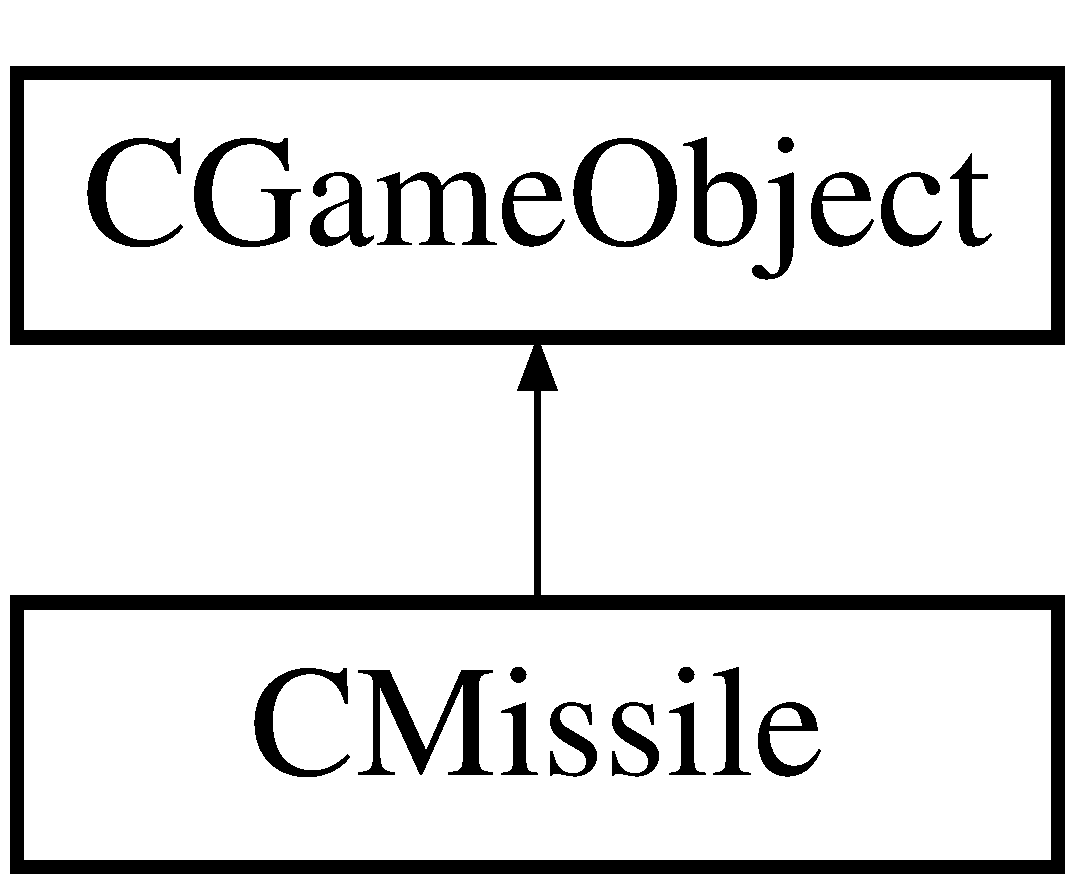
\includegraphics[height=2.000000cm]{class_c_missile}
\end{center}
\end{figure}
\subsection*{Public Member Functions}
\begin{DoxyCompactItemize}
\item 
\hyperlink{class_c_missile_a956f0b3cf58db39c91048b77410b66ef}{C\+Missile} ()
\begin{DoxyCompactList}\small\item\em contains intial object stats. \end{DoxyCompactList}\end{DoxyCompactItemize}
\subsection*{Additional Inherited Members}


\subsection{Detailed Description}
C++ Missile object contains missile data. 

This class has a all the characteristics of a Missile

\begin{DoxyAuthor}{Author}
Balkaran Sidhu 
\end{DoxyAuthor}


\subsection{Constructor \& Destructor Documentation}
\hypertarget{class_c_missile_a956f0b3cf58db39c91048b77410b66ef}{}\label{class_c_missile_a956f0b3cf58db39c91048b77410b66ef} 
\index{C\+Missile@{C\+Missile}!C\+Missile@{C\+Missile}}
\index{C\+Missile@{C\+Missile}!C\+Missile@{C\+Missile}}
\subsubsection{\texorpdfstring{C\+Missile()}{CMissile()}}
{\footnotesize\ttfamily C\+Missile\+::\+C\+Missile (\begin{DoxyParamCaption}{ }\end{DoxyParamCaption})}



contains intial object stats. 


\begin{DoxyParams}{Parameters}
{\em N\+O\+N\+E.} & \\
\hline
\end{DoxyParams}
\begin{DoxyReturn}{Returns}
nothing to return 
\end{DoxyReturn}


The documentation for this class was generated from the following files\+:\begin{DoxyCompactItemize}
\item 
C\+Missile.\+h\item 
C\+Missile.\+cpp\end{DoxyCompactItemize}

\hypertarget{class_c_ship}{}\section{C\+Ship Class Reference}
\label{class_c_ship}\index{C\+Ship@{C\+Ship}}


C++ ship object contains ship data.  




{\ttfamily \#include $<$C\+Ship.\+h$>$}

Inheritance diagram for C\+Ship\+:\begin{figure}[H]
\begin{center}
\leavevmode
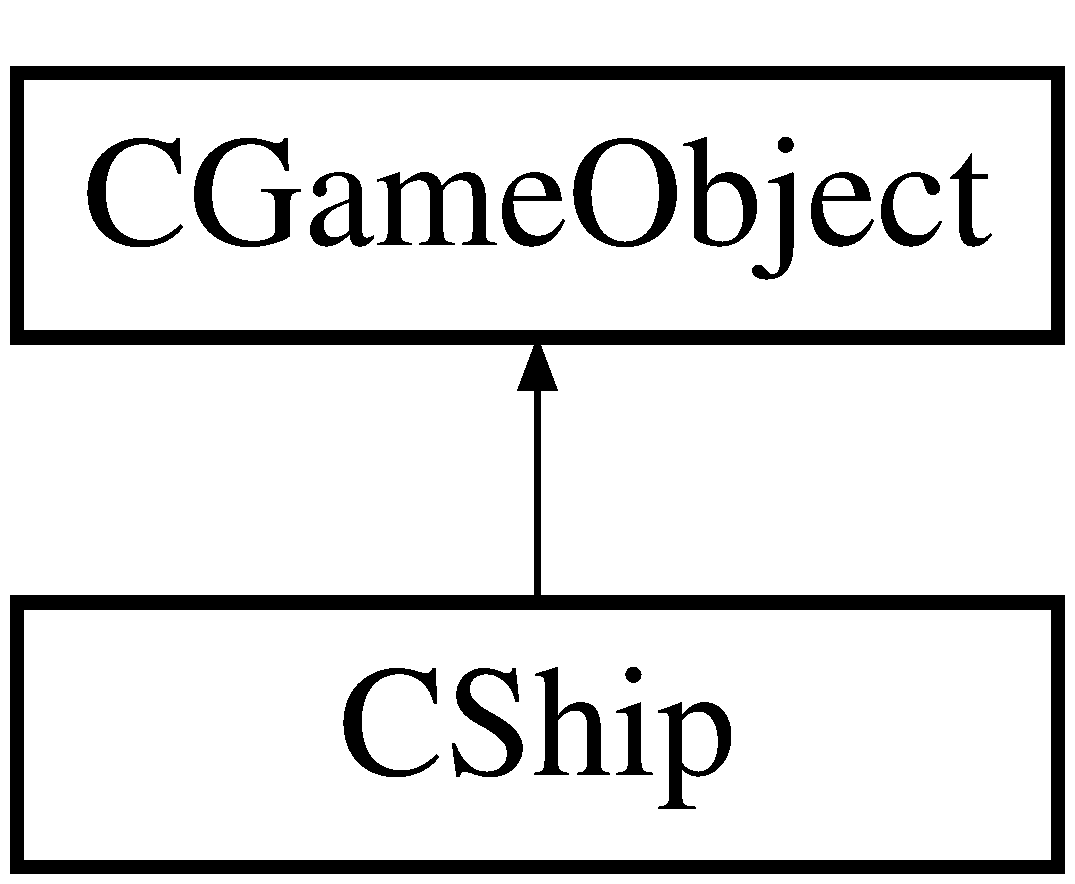
\includegraphics[height=2.000000cm]{class_c_ship}
\end{center}
\end{figure}
\subsection*{Public Member Functions}
\begin{DoxyCompactItemize}
\item 
\hyperlink{class_c_ship_ab360264b9bcbcd4b733a8b64cb8f7529}{C\+Ship} ()
\begin{DoxyCompactList}\small\item\em contains intial object stats. \end{DoxyCompactList}\end{DoxyCompactItemize}
\subsection*{Additional Inherited Members}


\subsection{Detailed Description}
C++ ship object contains ship data. 

This class has a all the characteristics of a ship

\begin{DoxyAuthor}{Author}
Balkaran Sidhu 
\end{DoxyAuthor}


\subsection{Constructor \& Destructor Documentation}
\hypertarget{class_c_ship_ab360264b9bcbcd4b733a8b64cb8f7529}{}\label{class_c_ship_ab360264b9bcbcd4b733a8b64cb8f7529} 
\index{C\+Ship@{C\+Ship}!C\+Ship@{C\+Ship}}
\index{C\+Ship@{C\+Ship}!C\+Ship@{C\+Ship}}
\subsubsection{\texorpdfstring{C\+Ship()}{CShip()}}
{\footnotesize\ttfamily C\+Ship\+::\+C\+Ship (\begin{DoxyParamCaption}{ }\end{DoxyParamCaption})}



contains intial object stats. 


\begin{DoxyParams}{Parameters}
{\em N\+O\+N\+E.} & \\
\hline
\end{DoxyParams}
\begin{DoxyReturn}{Returns}
nothing to return 
\end{DoxyReturn}


The documentation for this class was generated from the following files\+:\begin{DoxyCompactItemize}
\item 
C\+Ship.\+h\item 
C\+Ship.\+cpp\end{DoxyCompactItemize}

\hypertarget{class_serial}{}\section{Serial Class Reference}
\label{class_serial}\index{Serial@{Serial}}
\subsection*{Public Member Functions}
\begin{DoxyCompactItemize}
\item 
\hypertarget{class_serial_a599d3e220888815b8da436ea45a5c655}{}\label{class_serial_a599d3e220888815b8da436ea45a5c655} 
bool {\bfseries open} (std\+::string comm\+Port\+Name, int bit\+Rate=115200)
\item 
int \hyperlink{class_serial_aae3d630a4fd81c8b148cb4eebdb91392}{write} (const char $\ast$buffer, int buff\+Len)
\item 
int \hyperlink{class_serial_a8266889eb5bfa7ef8b53595c5482133d}{read} (char $\ast$buffer, int buff\+Len)
\item 
\hypertarget{class_serial_a63b7abf172cad25bfc998b3b1f98310f}{}\label{class_serial_a63b7abf172cad25bfc998b3b1f98310f} 
void {\bfseries flush} ()
\end{DoxyCompactItemize}


\subsection{Member Function Documentation}
\hypertarget{class_serial_a8266889eb5bfa7ef8b53595c5482133d}{}\label{class_serial_a8266889eb5bfa7ef8b53595c5482133d} 
\index{Serial@{Serial}!read@{read}}
\index{read@{read}!Serial@{Serial}}
\subsubsection{\texorpdfstring{read()}{read()}}
{\footnotesize\ttfamily int Serial\+::read (\begin{DoxyParamCaption}\item[{char $\ast$}]{buffer,  }\item[{int}]{buff\+Len }\end{DoxyParamCaption})}

Reads a string of bytes from the serial port.


\begin{DoxyParams}{Parameters}
{\em buffer} & pointer to the buffer to be written to \\
\hline
{\em buff\+Len} & the size of the buffer\\
\hline
\end{DoxyParams}
\begin{DoxyReturn}{Returns}
int the number of bytes read 
\end{DoxyReturn}
\hypertarget{class_serial_aae3d630a4fd81c8b148cb4eebdb91392}{}\label{class_serial_aae3d630a4fd81c8b148cb4eebdb91392} 
\index{Serial@{Serial}!write@{write}}
\index{write@{write}!Serial@{Serial}}
\subsubsection{\texorpdfstring{write()}{write()}}
{\footnotesize\ttfamily int Serial\+::write (\begin{DoxyParamCaption}\item[{const char $\ast$}]{buffer,  }\item[{int}]{buff\+Len }\end{DoxyParamCaption})}

Writes a string of bytes to the serial port.


\begin{DoxyParams}{Parameters}
{\em buffer} & pointer to the buffer containing the bytes \\
\hline
{\em buff\+Len} & the number of bytes in the buffer\\
\hline
\end{DoxyParams}
\begin{DoxyReturn}{Returns}
int the number of bytes written 
\end{DoxyReturn}


The documentation for this class was generated from the following files\+:\begin{DoxyCompactItemize}
\item 
Serial.\+h\item 
Serial.\+cpp\end{DoxyCompactItemize}

\hypertarget{class_server}{}\section{Server Class Reference}
\label{class_server}\index{Server@{Server}}
\subsection*{Public Member Functions}
\begin{DoxyCompactItemize}
\item 
\hypertarget{class_server_a7ebba75484fe844bb3e2920205455a74}{}\label{class_server_a7ebba75484fe844bb3e2920205455a74} 
void {\bfseries start} (int port)
\item 
\hypertarget{class_server_ad49615121ae4496bb6f8248530937101}{}\label{class_server_ad49615121ae4496bb6f8248530937101} 
void {\bfseries set\+\_\+txim} (cv\+::\+Mat \&im)
\item 
\hypertarget{class_server_ad01a77ea78115b7e6fc0603e0f239963}{}\label{class_server_ad01a77ea78115b7e6fc0603e0f239963} 
void {\bfseries get\+\_\+cmd} (std\+::vector$<$ std\+::string $>$ \&cmds)
\end{DoxyCompactItemize}


The documentation for this class was generated from the following files\+:\begin{DoxyCompactItemize}
\item 
server.\+h\item 
server.\+cpp\end{DoxyCompactItemize}

%--- End generated contents ---

% Index
\backmatter
\newpage
\phantomsection
\clearemptydoublepage
\addcontentsline{toc}{chapter}{Index}
\printindex

\end{document}
